% !TEX root = ../main.tex
\chapter{Quy trình xây dựng hệ thống (18 bước hiện thực)}

\section{Bước 1: Chuẩn bị môi trường và cấu hình trung tâm}

Hệ thống yêu cầu cài đặt môi trường ảo riêng biệt sử dụng công cụ quản lý gói tốc độ cao \texttt{uv} trên nền tảng Python 3.13, cố định phiên bản các thư viện trước khi tiến hành thực nghiệm:

\begin{lstlisting}[language=bash, caption={Khởi tạo môi trường ảo và cài đặt các gói phụ thuộc}]
# Cai dat uv neu chua co tren he thong
curl -LsSf https://astral.sh/uv/install.sh | sh

# Khoi tao va kich hoat moi truong ao Python 3.13
uv venv --python 3.13 .venv
source .venv/bin/activate  # Tren macOS/Linux

# Cai dat cac goi thu vien phu thuoc
uv pip install langgraph langchain langchain-core langchain-community \
               langchain-chroma chromadb rank-bm25 FlagEmbedding \
               pypdf pymupdf beautifulsoup4 fastapi uvicorn[standard] \
               langfuse ragas datasets pydantic python-dotenv requests
\end{lstlisting}

Toàn bộ tham số vận hành được tập trung tại \texttt{config.py}, tránh ghi cứng rải rác trong mã nguồn:

\begin{lstlisting}[language=Python, caption={Cấu hình trung tâm hệ thống trong config.py}]
import os
from pathlib import Path

BASE_DIR = Path(__file__).resolve().parent
DB_PATH = BASE_DIR / "app.db"
CHROMA_DIR = BASE_DIR / "data" / "processed" / "chroma"

# Nha cung cap LLM: "groq" | "openai" | "openrouter" | "ollama"
LLM_PROVIDER = os.getenv("LLM_PROVIDER", "groq")
LLM_MODEL = os.getenv("LLM_MODEL", "llama-3.3-70b-versatile")
LLM_TEMPERATURE = 0.0

EMBEDDING_MODEL = "BAAI/bge-m3"
RERANKER_MODEL = "BAAI/bge-reranker-v2-m3"

TOP_K_DENSE = 20
TOP_K_BM25 = 20
TOP_K_RERANK = 5

# Cap nguong quyet dinh CRAG (Toi uu hoa qua thuc nghiem quet luoi)
T_LOW = 0.35
T_HIGH = 0.70
INTERNAL_STRIP_MIN = 0.40
MAX_TOOL_ROUNDS = 3
HISTORY_TURNS = 6
\end{lstlisting}

\section{Bước 2: Tổ chức thư mục dự án}

Mã nguồn được cấu trúc theo nguyên lý phân tách trách nhiệm rõ ràng, chia tách giữa tác tử hội thoại và quy trình nạp tri thức:

\begin{lstlisting}[language=bash, caption={Cấu trúc cây thư mục chuẩn hóa của Legal CRAG Assistant}]
crag/
├── agent/                     # Dieu phoi luot hoi thoai va vong lap ReAct
│   ├── graph.py               # Dinh nghia StateGraph, routing va bien dich do thi
│   ├── state.py               # Dinh nghia AgentState va cac reducer channels
│   ├── nodes.py               # Logic xu ly tai Agent Node, Tool Node, Validator
│   ├── runtime.py             # Diem vao duy nhat: prepare_turn, persist_turn
│   └── context.py             # Context Manager lap ghep lich su va ho so client
├── retrieval/                 # Engine truy hoi da phuong thuc va tinh che
│   ├── dense.py               # Truy hoi vector ChromaDB voi mo hinh BGE-M3
│   ├── bm25.py                # Truy hoi tu khoa chinh xac rank-bm25
│   ├── fusion.py              # Thuat toan hop nhat hang RRF k=60
│   ├── reranker.py            # Cross-Encoder Reranker va chuan hoa Sigmoid
│   └── refine.py              # Boc tach legal strips va loc nguong phap ly
├── tools/                     # Bo cong cu tac tu theo OpenAPI Schema
│   ├── base.py                # Lop co so BaseLegalTool
│   ├── registry.py            # Quan ly dang ky va phan phoi cong cu
│   ├── crag_search.py         # Cong cu CRAG noi bo (Hybrid Search + Refinement)
│   └── web_search.py          # Cong cu tim kiem web voi whitelist cong quyen
├── legal/                     # Xu ly chuyen biet van ban quy pham phap luat
│   ├── cleaner.py             # Lam sach Unicode NFC, bo dot leaders, headers
│   ├── parser.py              # Phan tach cau truc Chuong, Dieu, Khoan, Diem
│   ├── citations.py           # Bo kiem dinh trich dan xac dinh (Citation Validator)
│   └── temporal.py            # Kiem tra hieu luc van ban theo thoi gian thuc
├── memory/                    # Quan ly bo nho phien va ho so nguoi dung
│   ├── store.py               # SQLite storage cho sessions, messages, memories
│   └── extractor.py           # Trich xuat thuoc tinh doanh nghiep theo Allow-List
├── ingestion/                 # Pipeline nap tri thuc tu dong 8 giai doan
│   ├── worker.py              # Background Worker ThreadPool chay da luong
│   ├── chunks.py              # Giai thuat Legal-aware Chunking giu tron Dieu
│   └── indexer.py             # Dong bo hoa Chroma vector va chi muc BM25
├── eval/                      # Bo danh gia kiem chuan khoa hoc
│   ├── run_eval.py            # Script do benchmark tu dong tren tap test
│   ├── metrics.py             # Cong thuc tinh RAGAS, Fallback va Citation
│   └── benchmark_report.json  # Bao cao ket qua dinh luong thuc te
├── api/                       # Ha tang FastAPI RESTful va SSE streaming
├── frontend/                  # Ung dung giao dien Next.js 14 SPA
├── schema.sql                 # DDL 8 bang quan he SQLite canonical
└── config.py                  # Cau hinh tham so tap trung toan he thong
\end{lstlisting}

\section{Bước 3: Chuẩn bị dữ liệu quy phạm pháp luật}

Dữ liệu được thu thập có chọn lọc từ Cổng Thông tin Điện tử Chính phủ (\texttt{chinhphu.vn}) và Cơ sở Dữ liệu Quốc gia về Văn bản Pháp luật (\texttt{vbpl.vn}), tập trung vào Luật Doanh nghiệp 2020, Bộ luật Lao động 2019 và các văn bản sửa đổi, bổ sung liên quan.

\begin{table}[htbp]
\centering
\caption{Quy mô dữ liệu quy phạm và các tập kiểm thử trong hệ thống}
\label{tab:corpus_scale}
\renewcommand{\arraystretch}{1.25}
\rowcolors{2}{tablerowalt}{white}
\begin{tabularx}{\textwidth}{L{6.0cm} Y}
\toprule
\rowcolor{tableheader}\color{white}\textbf{Thành phần dữ liệu} & \color{white}\textbf{Quy mô thực tế} \\
\midrule
Tổng số văn bản quy phạm thu thập & 27 văn bản (Luật, Nghị định, Thông tư, Văn bản hợp nhất) \\
Văn bản đã qua quy trình nạp đạt trạng thái READY & 15 văn bản chuẩn hóa hoàn chỉnh \\
Tổng số đoạn trích phân đoạn pháp lý (\textit{document\_chunks}) & 1.067 đoạn trích có tiêu đề ngữ cảnh \\
Tập dữ liệu hiệu chuẩn ngưỡng (\textit{Calibration Set}) & 20 câu hỏi có gán nhãn sự thật khách quan \\
Tập kiểm thử độc lập (\textit{Held-out Test Set}) & 40 câu hỏi phân bổ đều theo 5 nhóm nghiệp vụ \\
\bottomrule
\end{tabularx}
\end{table}

\section{Bước 4 \& 5: Thiết kế và khởi tạo cơ sở dữ liệu pháp lý SQLite}

Toàn bộ mô hình dữ liệu quan hệ được định nghĩa trong \texttt{schema.sql}, gồm 8 bảng phân chia giữa phân hệ nạp tri thức và phân hệ hội thoại:

\begin{lstlisting}[language=SQL, caption={Trích đoạn DDL lược đồ cơ sở dữ liệu SQLite app.db}]
PRAGMA foreign_keys = ON;

-- 1. Quan ly danh muc van ban phap ly goc
CREATE TABLE IF NOT EXISTS documents (
    id TEXT PRIMARY KEY,
    filename TEXT NOT NULL,
    document_number TEXT,
    title TEXT NOT NULL,
    document_type TEXT,
    issuing_authority TEXT,
    effective_from DATE,
    effective_to DATE,
    status TEXT NOT NULL DEFAULT 'UPLOADED', -- UPLOADED | PROCESSING | READY | FAILED
    legal_status TEXT NOT NULL DEFAULT 'effective', -- effective | expired | partially_expired
    content_hash TEXT,
    chunk_count INTEGER DEFAULT 0,
    created_at TEXT DEFAULT CURRENT_TIMESTAMP
);

-- 2. Cac doan trich phan manh phap ly (don vi truy hoi co so)
CREATE TABLE IF NOT EXISTS document_chunks (
    id TEXT PRIMARY KEY,
    document_id TEXT NOT NULL,
    chunk_index INTEGER NOT NULL,
    chapter TEXT, article TEXT, clause TEXT, point TEXT,
    heading TEXT,
    page_start INTEGER, page_end INTEGER,
    content TEXT NOT NULL,
    token_count INTEGER,
    FOREIGN KEY(document_id) REFERENCES documents(id) ON DELETE CASCADE
);

-- 3. Quan he sua doi, bo sung, thay the giua cac van ban
CREATE TABLE IF NOT EXISTS legal_relations (
    id INTEGER PRIMARY KEY AUTOINCREMENT,
    source_document_id TEXT NOT NULL,
    target_document_id TEXT NOT NULL,
    relation_type TEXT NOT NULL, -- 'amends', 'supplements', 'replaces', 'repeals', 'guides'
    note TEXT,
    FOREIGN KEY(source_document_id) REFERENCES documents(id) ON DELETE CASCADE,
    FOREIGN KEY(target_document_id) REFERENCES documents(id) ON DELETE CASCADE
);

-- 4. Tien trinh xu ly nap du lieu cua quan tri vien
CREATE TABLE IF NOT EXISTS ingestion_jobs (
    id TEXT PRIMARY KEY,
    document_id TEXT NOT NULL,
    stage TEXT NOT NULL DEFAULT 'PARSING',
    progress REAL NOT NULL DEFAULT 0.0,
    detail TEXT,
    FOREIGN KEY(document_id) REFERENCES documents(id) ON DELETE CASCADE
);
\end{lstlisting}

\section{Bước 6: Cấu hình LLM đa nhà cung cấp, mô hình nhúng và xếp hạng lại}

Module \texttt{llm.py} cài đặt mô hình Factory Pattern hỗ trợ đa nhà cung cấp, đảm bảo tính sẵn sàng cao với cơ chế chuyển đổi dự phòng tự động:

\begin{lstlisting}[language=Python, caption={Khởi tạo mô hình ngôn ngữ, mô hình nhúng và xếp hạng lại}]
# llm.py
from config import LLM_PROVIDER, LLM_MODEL, LLM_TEMPERATURE

def get_chat_model(provider: str = None, model: str = None):
    p = (provider or LLM_PROVIDER).lower()
    m = model or LLM_MODEL
    if p == "groq":
        from langchain_groq import ChatGroq
        return ChatGroq(model=m, temperature=LLM_TEMPERATURE)
    elif p == "openai":
        from langchain_openai import ChatOpenAI
        return ChatOpenAI(model=m, temperature=LLM_TEMPERATURE)
    elif p == "ollama":
        from langchain_ollama import ChatOllama
        return ChatOllama(model=m, temperature=LLM_TEMPERATURE)
    # OpenRouter va logic chuyen doi du phong...

# Khoi tao mo hinh nhung da ngu BAAI/bge-m3 (vector 1024 chieu)
from langchain_ollama import OllamaEmbeddings
embeddings = OllamaEmbeddings(model="bge-m3")

# retrieval/reranker.py: Mo hinh Cross-Encoder BAAI/bge-reranker-v2-m3
from FlagEmbedding import FlagReranker
from math import exp

reranker = FlagReranker("BAAI/bge-reranker-v2-m3", use_fp16=True)

def sigmoid(z: float) -> float:
    return 1.0 / (1.0 + exp(-float(z)))

def rerank(query: str, docs: list[dict], top_k: int = 5) -> list[dict]:
    if not docs:
        return []
    pairs = [[query, d.get("content", d.get("text", ""))] for d in docs]
    raw_scores = reranker.compute_score(pairs)
    scored = []
    for doc, s in zip(docs, raw_scores):
        doc_copy = dict(doc)
        doc_copy["score"] = sigmoid(s)
        scored.append(doc_copy)
    return sorted(scored, key=lambda x: x["score"], reverse=True)[:top_k]
\end{lstlisting}

\section{Bước 7: Định nghĩa trạng thái tác tử với các bộ tích lũy}

Để duy trì quỹ đạo ReAct nhiều lượt và thu thập chứng cứ không bị ghi đè, \texttt{AgentState} được định nghĩa với các bộ tích lũy chuyên dụng:

\begin{lstlisting}[language=Python, caption={Định nghĩa trạng thái AgentState trong agent/state.py}]
import operator
from typing import Annotated, Any, Dict, List, Optional, TypedDict
from langchain_core.messages import BaseMessage
from langgraph.graph.message import add_messages

class AgentState(TypedDict, total=False):
    # Thong tin yeu cau va ngu canh hoi thoai
    client_id: str
    session_id: str
    query: str
    as_of_date: Optional[str]
    memory_context: str
    conversation_history: str

    # Quy dao suy luan ReAct (Tich luy qua cac luot goi cong cu)
    messages: Annotated[List[BaseMessage], add_messages]
    evidence: Annotated[List[Dict[str, Any]], operator.add]
    tool_trace: Annotated[List[Dict[str, Any]], operator.add]

    # Ket qua sinh va kiem dinh trich dan
    generation: Dict[str, Any]       # {"answer": str, "claims": [...], "abstain": bool}
    citation_report: Dict[str, Any]  # Ket qua tu CitationValidator
    follow_up_questions: List[str]   # Goi y cau hoi tiep theo
    trace_meta: Dict[str, Any]
\end{lstlisting}

\section{Bước 8: Quy trình nạp dữ liệu và phân đoạn pháp lý}

Quy trình nạp tài liệu tự động gồm 8 giai đoạn khép kín, được minh họa chi tiết tại Hình~\ref{fig:ingestion_pipeline}.

\begin{figure}[htbp]
    \centering
    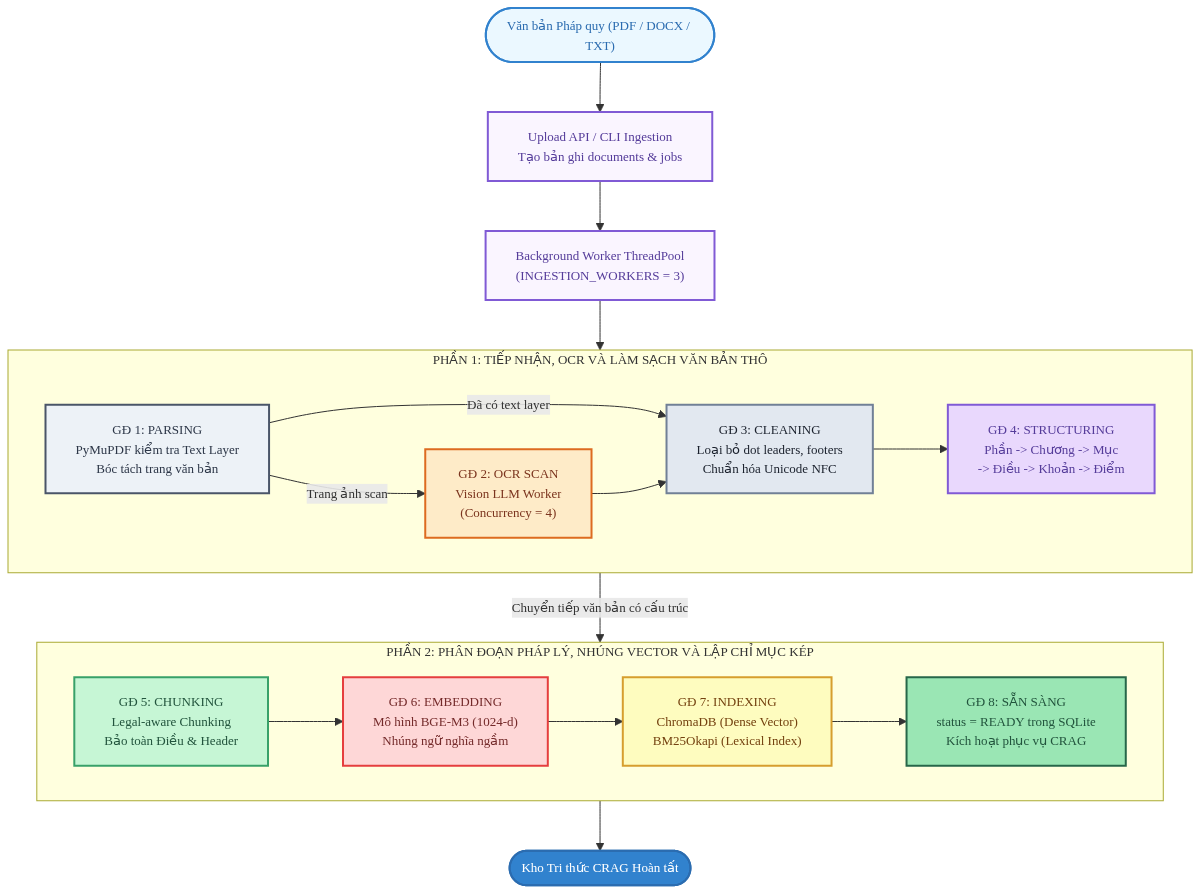
\includegraphics[width=\textwidth]{images/ingestion_pipeline.png}
    \caption{Quy trình 8 giai đoạn nạp dữ liệu tự động từ tệp văn bản thô đến chỉ mục kép Chroma và BM25.}
    \label{fig:ingestion_pipeline}
\end{figure}

Tiến trình xử lý được chia thành:
\begin{enumerate}
    \item \textbf{Phân tích cú pháp và nhận dạng quang học:} Nhận diện tệp Word hoặc PDF. Các trang quét ảnh scan được bóc tách và nạp qua Vision LLM OCR với mức song song $\text{OCR\_CONCURRENCY} = 4$.
    \item \textbf{Làm sạch và cấu trúc hóa:} Loại bỏ biểu mẫu chấm, tiêu đề đầu trang và chân trang, chuẩn hóa bảng mã Unicode tiếng Việt NFC và nhận diện thứ bậc quy phạm pháp luật (\textit{Phần $\to$ Chương $\to$ Mục $\to$ Điều $\to$ Khoản $\to$ Điểm}).
    \item \textbf{Phân đoạn pháp lý bảo toàn ngữ cảnh:} Phân đoạn ngữ nghĩa điều luật bảo toàn ranh giới (Hình~\ref{fig:legal_chunking_flow}).
    \item \textbf{Nhúng vector và lập chỉ mục:} Tạo vector ngữ nghĩa BGE-M3 lưu vào ChromaDB và cập nhật chỉ mục từ khóa BM25Okapi dưới nền.
\end{enumerate}

\begin{figure}[htbp]
    \centering
    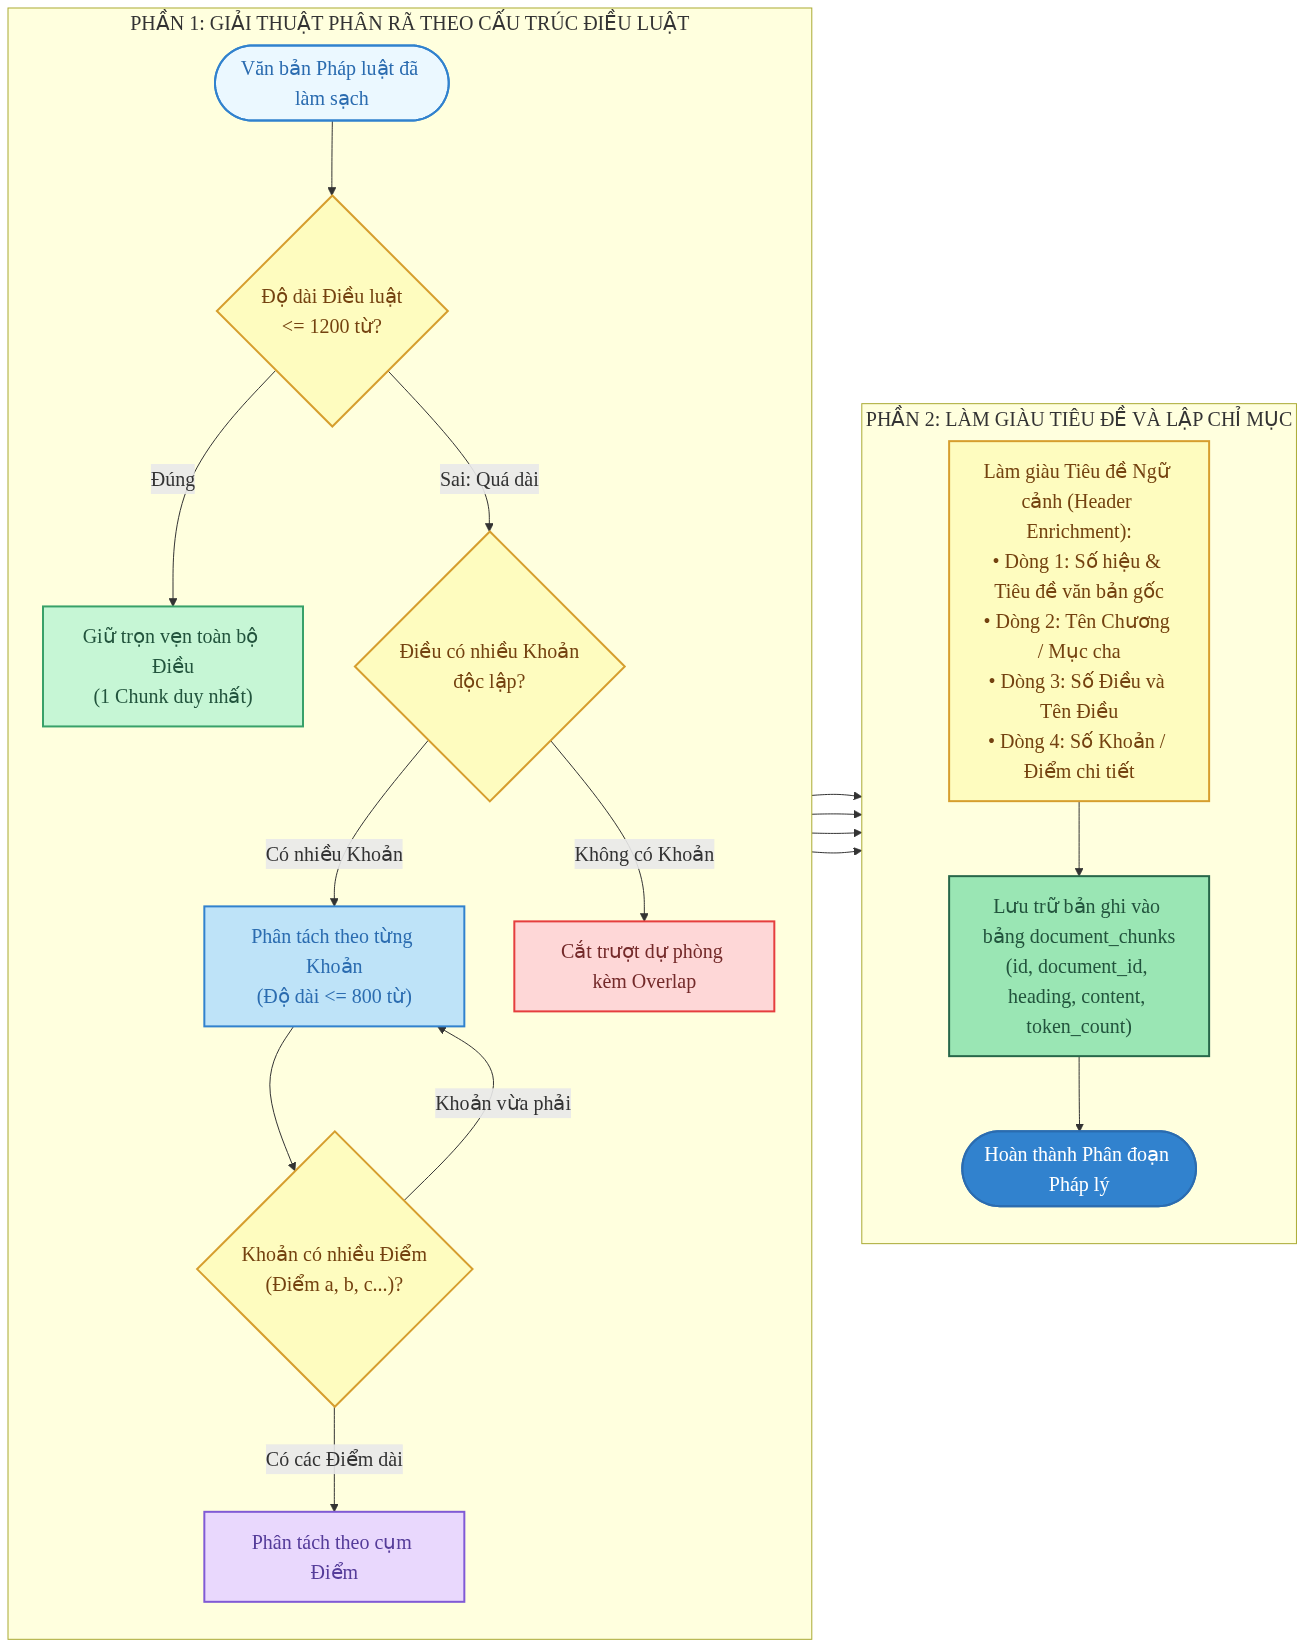
\includegraphics[width=0.88\textwidth]{images/legal_chunking_flow.png}
    \caption{Giải thuật phân đoạn pháp lý Legal-aware Chunking: Bảo toàn nguyên vẹn Điều luật và làm giàu tiêu đề ngữ cảnh.}
    \label{fig:legal_chunking_flow}
\end{figure}

Giải thuật phân đoạn pháp lý tuân thủ nguyên tắc:
\begin{itemize}
    \item Nếu Điều luật $\le 1200$ từ: Giữ nguyên vẹn toàn bộ Điều thành một đoạn trích duy nhất nhằm bảo toàn tính thống nhất giữa các khoản quy định.
    \item Nếu Điều luật $> 1200$ từ: Phân tách theo từng Khoản độc lập; nếu Khoản vẫn quá dài thì tiếp tục bóc tách theo cụm Điểm.
    \item \textbf{Làm giàu tiêu đề ngữ cảnh:} Mỗi đoạn trích đều được gắn kèm dòng tiêu đề ngữ cảnh phân cấp: \textit{Số hiệu văn bản $\to$ Tên Chương/Mục $\to$ Tên Điều $\to$ Số Khoản/Điểm}.
\end{itemize}

\section{Bước 9: Hệ thống quản trị công cụ và cơ chế điều phối}

Module \texttt{tools/registry.py} quản lý danh mục công cụ, chuyển đổi tự động sang cấu trúc lược đồ chuẩn để mô hình ngôn ngữ lớn thực hiện cơ chế gọi hàm (\textit{function calling}) một cách chuẩn xác.

\section{Bước 10: Động cơ truy hồi CRAG và bộ đánh giá ba nhánh}

Công cụ \texttt{crag\_search} là trọng tâm của kỹ thuật Corrective RAG trong hệ thống, thực hiện quy trình xử lý khép kín mô tả tại Hình~\ref{fig:crag_retrieval_branches}.

\begin{figure}[htbp]
    \centering
    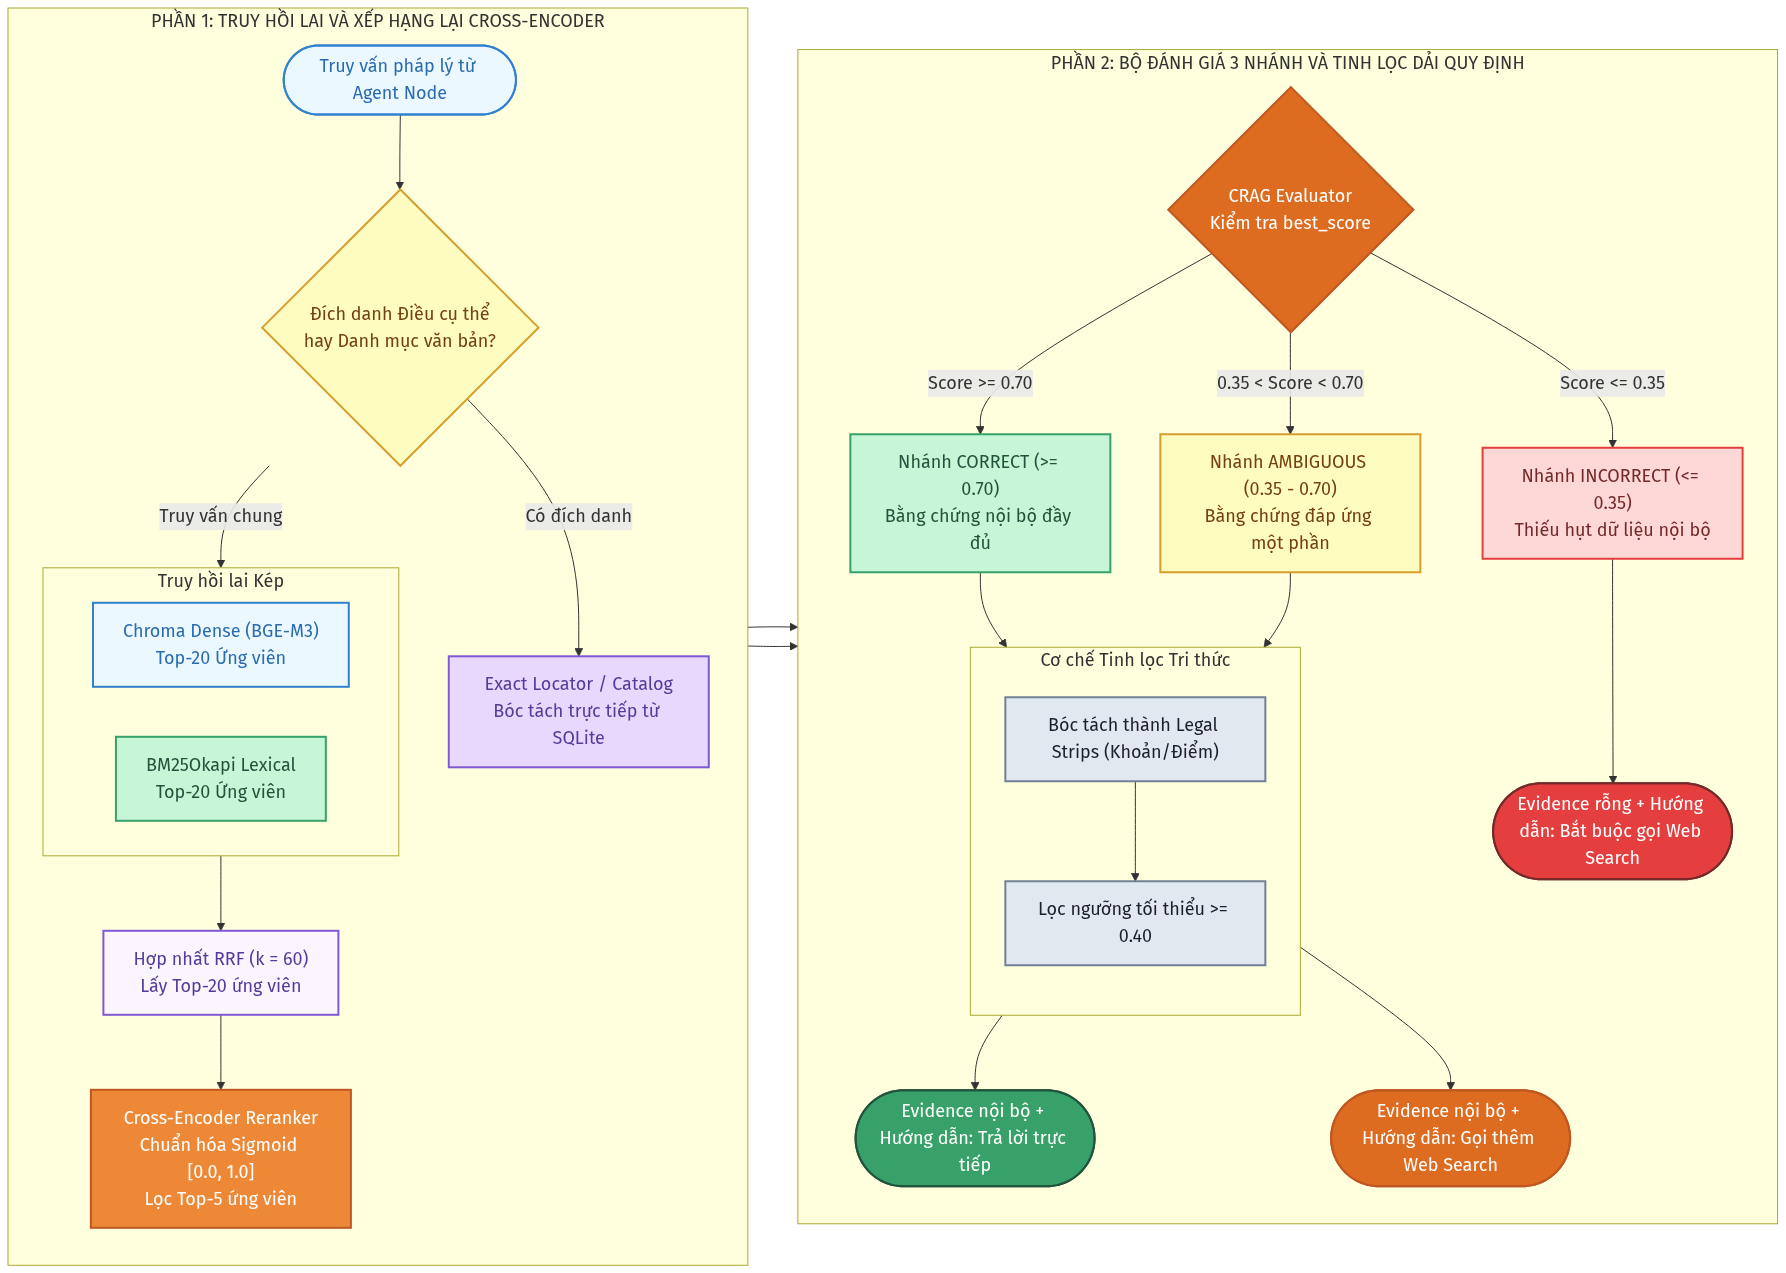
\includegraphics[width=\textwidth]{images/crag_retrieval_branches.png}
    \caption{Luồng xử lý chi tiết bên trong công cụ crag\_search và cơ chế rẽ ba nhánh điều kiện của CRAG.}
    \label{fig:crag_retrieval_branches}
\end{figure}

\subsection{Truy hồi lai và hợp nhất thứ hạng RRF}
Hệ thống truy hồi đồng thời 20 ứng viên hàng đầu từ Chroma (Dense) và 20 ứng viên từ BM25 (Lexical), sau đó hợp nhất bằng giải thuật Reciprocal Rank Fusion với hằng số làm mịn $k = 60$:
\begin{equation}
S_{\text{RRF}}(d) = \sum_{r \in \{\text{Dense}, \text{BM25}\}} \frac{1}{60 + \text{rank}_r(d)}
\end{equation}

\subsection{Đánh giá và rẽ ba nhánh điều kiện CRAG}
Danh sách 5 ứng viên hàng đầu sau khi xếp hạng lại bằng Cross-Encoder được đưa qua hàm đánh giá ngưỡng:
\begin{equation}
\text{Action} = \begin{cases}
\mathbf{CORRECT} & \text{nếu } \max(S) \ge T_{high} \;(0.70) \\
\mathbf{INCORRECT} & \text{nếu } \max(S) \le T_{low} \;(0.35) \\
\mathbf{AMBIGUOUS} & \text{nếu } T_{low} < \max(S) < T_{high}
\end{cases}
\end{equation}

\subsection{Cơ chế tinh lọc tri thức (Knowledge Refinement)}
Khi nhánh rẽ là \textbf{CORRECT} hoặc \textbf{AMBIGUOUS}, hệ thống kích hoạt \texttt{refine\_internal}:
\begin{enumerate}
    \item Phân rã từng đoạn văn bản thành các dải quy định cụ thể (\textit{legal strips} theo từng Khoản hoặc Điểm).
    \item Chấm lại điểm liên quan của từng dải quy định bằng mô hình Cross-Encoder.
    \item Lọc bỏ toàn bộ các dải quy định có điểm số dưới ngưỡng tối thiểu $\text{INTERNAL\_STRIP\_MIN} = 0.40$.
\end{enumerate}

\section{Bước 11: Tìm kiếm web có kiểm soát}

Khi kho dữ liệu nội bộ không có căn cứ phù hợp (\textbf{INCORRECT}) hoặc chỉ đáp ứng một phần (\textbf{AMBIGUOUS}), tác tử tự động gọi công cụ tìm kiếm web với danh mục tên miền cho phép:
\begin{lstlisting}[language=Python, caption={Bộ lọc tên miền chính thống cho công cụ tìm kiếm web}]
OFFICIAL_DOMAINS = {
    "vbpl.vn", "vanban.chinhphu.vn", "moj.gov.vn", 
    "chinhphu.vn", "thuvienphapluat.vn", "congbao.chinhphu.vn"
}

def is_allowed_source(url: str) -> bool:
    try:
        host = url.lower().split("/")[2]
        return any(host == d or host.endswith("." + d) for d in OFFICIAL_DOMAINS)
    except Exception:
        return False
\end{lstlisting}

\section{Bước 12: Bộ kiểm định trích dẫn xác định}

Module \texttt{legal/citations.py} đóng vai trò chốt chặn an toàn cuối cùng trước khi phản hồi được xuất ra cho người dùng:
\begin{enumerate}
    \item \textbf{Kiểm tra tính tồn tại của căn cứ:} Mọi mã trích dẫn \texttt{[source\_id]} xuất hiện trong câu trả lời phải nằm trong tập bằng chứng (\textit{evidence map}) đã được thu thập thực tế.
    \item \textbf{Kiểm tra tính hiệu lực theo thời gian:} Căn cứ vào ngày tham chiếu \texttt{as\_of\_date}, hệ thống đối chiếu với trường \texttt{effective\_from}, \texttt{effective\_to} và quan hệ bãi bỏ/thay thế trong cơ sở dữ liệu để cảnh báo nếu trích dẫn văn bản đã hết hiệu lực.
    \item \textbf{Cơ chế từ chối an toàn (Safe Abstain):} Nếu phát hiện trích dẫn giả mạo hoặc không có căn cứ, hệ thống tự động gắn cờ \texttt{abstain = true} và thay thế bằng câu trả lời an toàn chuẩn: \textit{“Chưa đủ căn cứ pháp lý để kết luận.”}
\end{enumerate}

\section{Bước 13: Thiết kế câu lệnh nhắc sinh phản hồi có cấu trúc JSON}

Mô hình ngôn ngữ được ràng buộc tuân thủ khuôn dạng đầu ra có cấu trúc nhằm phân tách rõ rệt giữa mệnh đề kết luận và mã nguồn trích dẫn:

\begin{lstlisting}[caption={Câu lệnh nhắc sinh câu trả lời có cấu trúc nghiêm ngặt}]
Bạn là trợ lý hỗ trợ tra cứu tuân thủ pháp lý doanh nghiệp.
Chỉ trả lời dựa duy nhất trên các căn cứ pháp lý hiện tại được cung cấp dưới đây.

Yêu cầu bắt buộc:
1. Tuyệt đối không tự suy đoán hoặc sáng tạo quy định pháp luật.
2. Mọi kết luận pháp lý phải được gắn kèm [source_id] của bằng chứng tương ứng.
3. Nếu chưa đủ căn cứ, trả lời rõ ràng: "Chưa đủ căn cứ pháp lý để kết luận."
4. Định dạng đầu ra: Bắt buộc trả về đúng định dạng JSON Schema:
   {
     "answer": "Nội dung giải thích súc tích...",
     "claims": [
       {"text": "Mệnh đề pháp lý 1", "source_ids": ["E1", "E2"]},
       {"text": "Mệnh đề pháp lý 2", "source_ids": ["E3"]}
     ],
     "abstain": false
   }

Căn cứ pháp lý:
{evidence_context}

Câu hỏi:
{query}
\end{lstlisting}

\section{Bước 14: Xây dựng và biên dịch đồ thị LangGraph ReAct}

Lõi điều phối được lập trình trong \texttt{agent/graph.py} với đồ thị trạng thái 3 nút chính:

\begin{lstlisting}[language=Python, caption={Thiết lập đồ thị LangGraph ReAct trong agent/graph.py}]
from langgraph.graph import StateGraph, START, END
from agent.state import AgentState
from agent.nodes import agent_node, route_after_agent, tool_node, validate_citations_node

def build_crag_graph():
    g = StateGraph(AgentState)
    
    # Ba nut chinh cua chu trinh ReAct
    g.add_node("agent", agent_node)
    g.add_node("tools", tool_node)
    g.add_node("cite_validate", validate_citations_node)
    
    g.add_edge(START, "agent")
    
    # Canh dieu kien phan nhanh sau khi Agent suy luan
    g.add_conditional_edges(
        "agent",
        route_after_agent,
        {
            "tools": "tools",                   # LLM yeu cau goi cong cu
            "agent": "agent",                   # Tiep tuc suy luan
            "cite_validate": "cite_validate"    # Hoan tat, chuyen sang kiem dinh
        }
    )
    
    g.add_edge("tools", "agent")                # Observation tra ve cho Agent
    g.add_edge("cite_validate", END)            # Ket thuc luot hoi thoai
    
    return g.compile()
\end{lstlisting}

\section{Bước 15: Kịch bản kiểm thử thực nghiệm phục vụ trình diễn}

Hệ thống cung cấp sẵn kịch bản kiểm thử tự động \texttt{python main.py --demo} bao phủ 5 tình huống kiểm thử đại diện (Bảng~\ref{tab:demo_tests}).

\begin{table}[htbp]
\centering
\caption{Năm kịch bản kiểm thử bắt buộc cần minh chứng hoạt động của CRAG}
\label{tab:demo_tests}
\renewcommand{\arraystretch}{1.25}
\rowcolors{2}{tablerowalt}{white}
\begin{tabularx}{\textwidth}{C{1.8cm} L{4.0cm} Y}
\toprule
\rowcolor{tableheader}\color{white}\textbf{Kịch bản} & \color{white}\textbf{Tình huống kiểm thử} & \color{white}\textbf{Luồng xử lý kỳ vọng của hệ thống} \\
\midrule
\textbf{Kịch bản 1} & \textit{Correct Case:} Câu hỏi trong kho có đầy đủ căn cứ nội bộ. & Điểm số $\ge 0.70 \;\to\; \mathbf{CORRECT} \;\to\; \text{Tinh lọc dải quy định} \;\to\; \text{Sinh phản hồi} \;\to\; \text{Kiểm định trích dẫn}$. \\
\textbf{Kịch bản 2} & \textit{Incorrect Case:} Câu hỏi về nghị định mới chưa nạp vào kho dữ liệu. & Điểm số $\le 0.35 \;\to\; \mathbf{INCORRECT} \;\to\; \text{Viết lại truy vấn} \;\to\; \text{Tìm kiếm web chính thống} \;\to\; \text{Sinh phản hồi}$. \\
\textbf{Kịch bản 3} & \textit{Ambiguous Case:} Kho nội bộ có quy định khung nhưng thiếu thủ tục chi tiết. & $0.35 < \text{Điểm} < 0.70 \;\to\; \mathbf{AMBIGUOUS} \;\to\; \text{Tinh lọc} + \text{Web} \;\to\; \text{Hợp nhất bằng chứng} \;\to\; \text{Sinh phản hồi}$. \\
\textbf{Kịch bản 4} & \textit{Exact Locator:} “Điều 25 Bộ luật Lao động 2019 quy định gì?” & Cơ chế định vị trực tiếp bóc tách toàn bộ các Khoản từ SQLite $\;\to\;$ Phản hồi chính xác tuyệt đối. \\
\textbf{Kịch bản 5} & \textit{Citation Guardrail:} Mô hình cố tình trích dẫn nguồn không có thật. & Bộ kiểm định phát hiện mã trích dẫn giả mạo $\;\to\;$ Thiết lập \texttt{abstain = true} chặn đứng ảo giác. \\
\bottomrule
\end{tabularx}
\end{table}
